\entry{Semana del 23/06/2025}
\section{Lunes 23/06/2025}

\subsection*{Notas rápidas del día:}
\begin{itemize}
	\item Con la pinza agarrando el esmalte, tornillo más abajo de todo y 4 cm de agua (+ 1 cm de cuba) daba 53.576 kHz de fase 0°.
	\item Ahora agarrando bien está en 52.579 kHz.
	\item ¿Olor a quemado?. 
	
	\item Resistencia de 11/12 Ohm. 52.761 Khz.
	\item Ahora 53.214 kHz.
\end{itemize}

Me centré en terminar un par de cosas de código, especialmente integrar en la interfaz poder elegir la ganancia de cada canal, que eso se guarde en los metadatos y después se tenga en cuenta al convertir los datos binarios, ya que el voltaje máximo se verá limitado a $\pm10$ V/\textit{gain}, o en su defecto de 0 a 10V/\textit{gain} si está configurado en Unipolar.

Las posibles ganancias para este dispositivo son x1, x2, x5, x10, x50 y x100, y definimos en \textit{daqh} las flagas correspondientes bajo el nombre de \textbf{daqh.DgainPS3kX1} y demás.

\begin{figure}[th!]
	\centering
	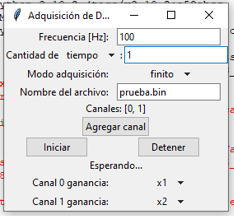
\includegraphics[width=0.27456\linewidth]{Figures/23_06_2025/Ganancias}
	\caption{Nueva interfaz con posibilidad de elegir la ganancia de cada canal.}
	\label{fig:ganancias}
\end{figure}



La idea de poder usar la ganancia hasta x100 era poder usar resistencias más bajas, sobre las que va a caer menor potencial y necesitamos más resolución para definirlas bien, pero volví a probar con forzados y gotas de agua y el ruido seguía estando aún con ganancia x100 en ese canal. Por ahí el ruido es eléctrico y también termina siendo amplificado.

\begin{figure}[th!]
	\centering
	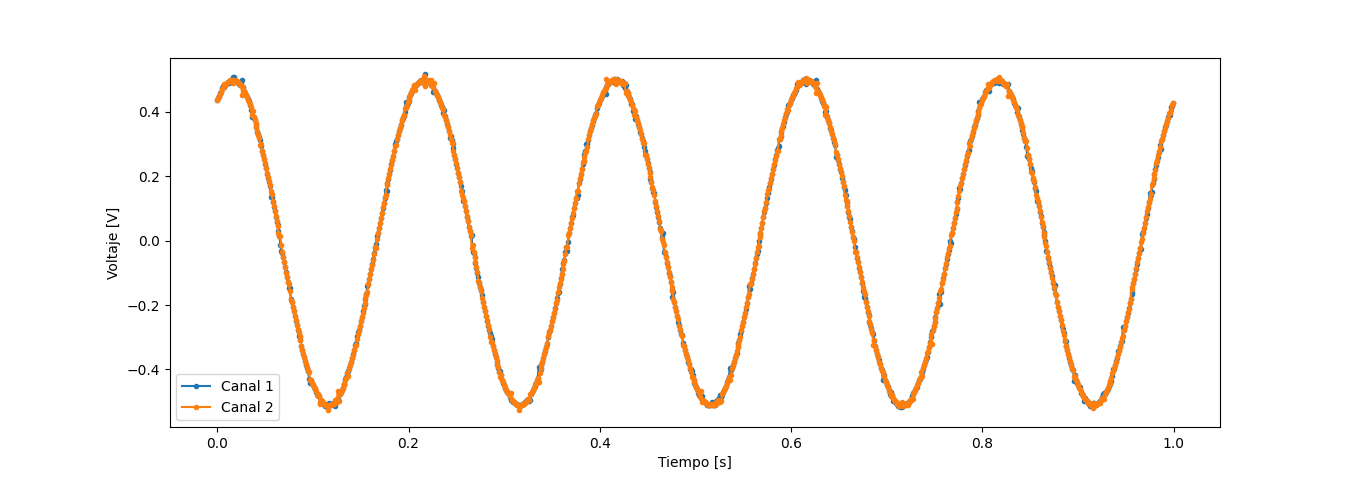
\includegraphics[width=0.87\linewidth]{Figures/23_06_2025/Ganancia_x10_canal2}
	\caption{Misma señal capturada con ganancia x1 en el canal 1 y x10 en el canal 2, a 1kHz de sampleo.}
	\label{fig:gananciax10canal2}
\end{figure}


Además pasé a usar en el graficador a tiempo real el filtro exponencial para pasar a la siguiente iteración los últimos valores de la anterior y que no de los saltos de los primeros puntos cada vez, mejorando bastante el ruido y permitiendo elegir más puntos de la secuencia para graficar y no solo el último o un promedio.

\begin{figure}[th!]
	\centering
	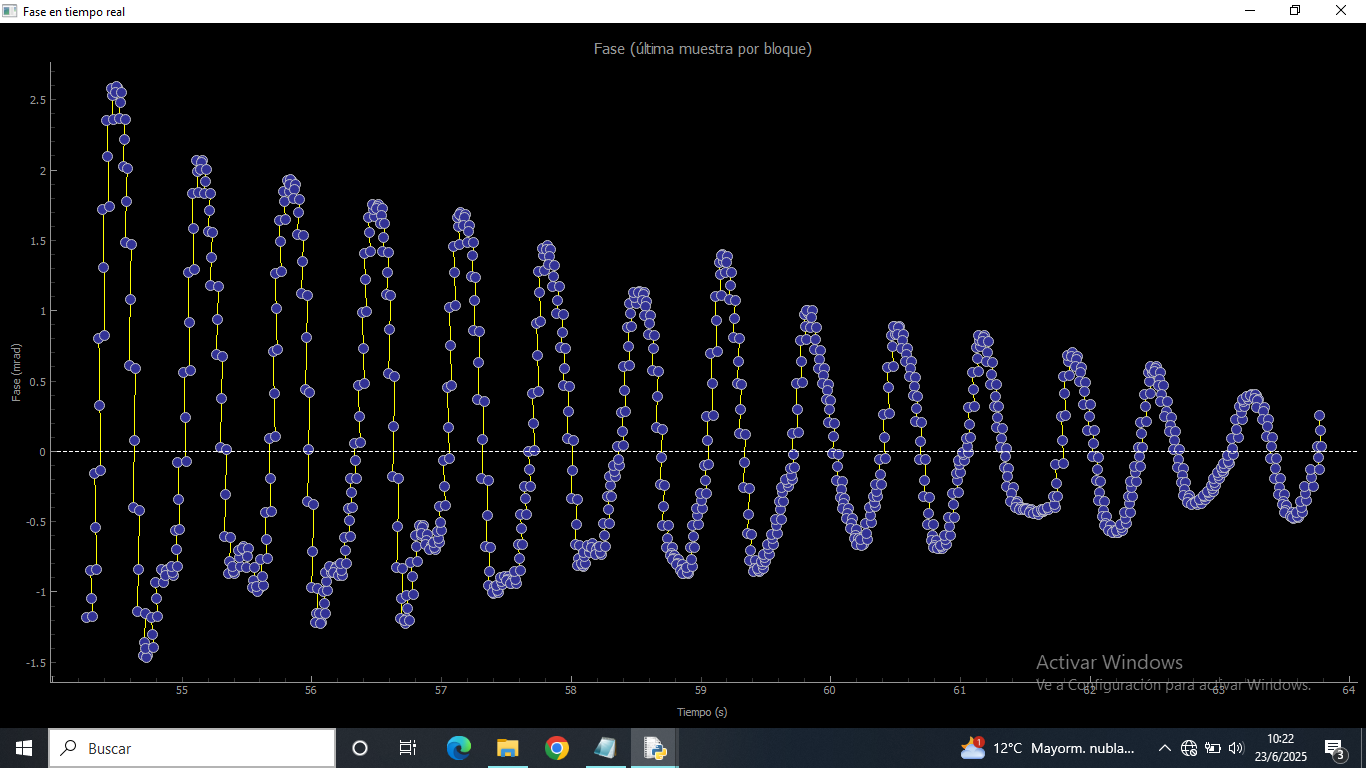
\includegraphics[width=0.567\linewidth]{Figures/23_06_2025/Mejor_tiempo_real}
	\caption{Ejemplo de oscilaciones en tiempo real con el filtro exponencial.}
	\label{fig:mejortiemporeal}
\end{figure}

Durante estas mejoras de código empecé a sentir olor a quemado recurrentemente así que terminé desarmando todo por no poder identificar la fuente y al salir del Labo me di cuenta que era de afuera por algún arreglo que estaban haciendo cortando metal con soplete. 

También Manu forzó la cuba chica para probar tomar una medición de turbulencias de ondas típica, la serie temporal resultó ser como se esperaría:

\begin{figure}[th!]
	\centering
	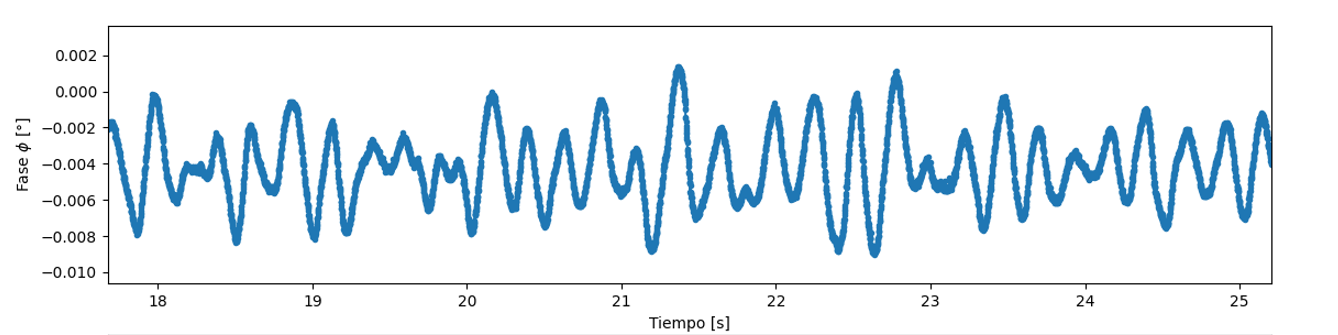
\includegraphics[width=0.87\linewidth]{Figures/23_06_2025/Forzado_Manu_Lunes}
	\caption{Forzado manual de la cuba chica, serie temporal obtenida con el sensor+lock-in.}
	\label{fig:forzadomanulunes}
\end{figure}

Para analizar esto partí la señal de 60 segundos en 6 partes y tomé promedios de las ffts al cuadrado de cada una (PSD). 



\begin{figure}[th!]
	\centering
	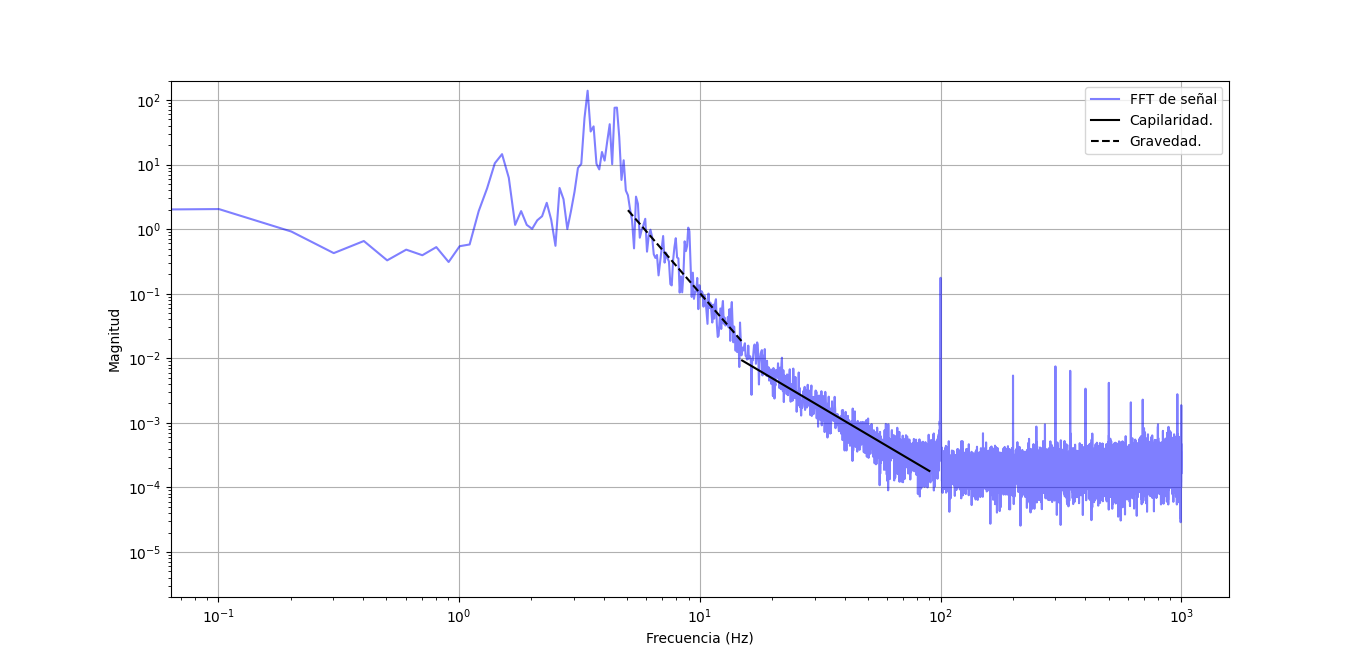
\includegraphics[width=0.7\linewidth]{Figures/23_06_2025/Espectro_Manu_Lunes}
	\caption{Espectro promedioado del forzado en la cuba chica (log-log) con ajustes en ambos rangos.}
	\label{fig:espectromanulunes}
\end{figure}

Ajusté el espectro antes de 15 Hz por un lado y después hasta más o menos 90 Hz por otro para saber qué pendientes habían en esos rangos (gravedad y capilar) en log-log y saber si aparecían las leyes de potencias.

Los resultados del ajuste fueron:
\begin{itemize}
	\item Gravedad: $m=-(4.3\pm0.2)$ rad$^2$/Hz$^2$, $b=(7.6\pm0.4)$ rad$^2$/Hz, $R^2=-0.92029$. 
	\item Capilar: $m=-(2.20\pm0.03)$ rad$^2$/Hz$^2$, $b=(1.3\pm0.1)$ rad$^2$/Hz, $R^2=-0.92283$.
\end{itemize}

Las pendientes son cercanas a las que esperaríamos, -4 para gravedad y -17/6 para capilar, pero no estoy del todo seguro porqué el $R^2$ de \textit{linregress} de Scipy da negativo.

La frecuencia de cruce termina dando aproximadamente 20 Hz, y debería ser creo 17 Hz.

Pablo después sugirió usar la función \textbf{Welch} de Scipy que calcula directamente la PSD en ventanas de la señal total con cierto overlap y las promedia todas. Además dividir por lo esperado para tratar de identificar mesentas o plateaus.

Y después para la PDF de las alturas el histograma de las alturas, suavizaado con kde\_gaussian de scipy. % y 

\begin{figure}[th!]
	\centering
	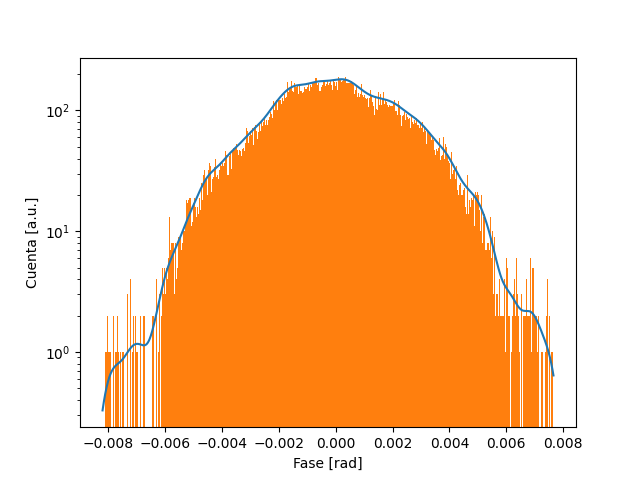
\includegraphics[width=0.4567\linewidth]{Figures/23_06_2025/PDFs_Manu_Lunes}
	\caption{Histograma de las alturas con 1000 bins y kde\_gaussian de Scipy.}
	\label{fig:pdfsmanulunes}
\end{figure}

\section{Miércoles 25/06/2025}

\subsection*{Notas rápidas del día:}
\begin{itemize}
	\item Empiezo pruebas iniciales con agua de la canilla antes de probar la del canal. Resistencia 1.8kOhm, 3.7 cm de altura de agua. 
	\item Queda siempre algún contacto medio suelto, no sé si en la protoboard o que se tocan los alambres, pero hasta no arreglar eso el sensor no suele funcionar correctamente. Por ejemplo, recién daba 53.6 kHz de resonancia pero no había oscilaciones al mover el agua, y después de tocar un pcoo los componentes dio un salto y la fase 0° está en 51.829 kHz y sí hay oscilaciones notables al mover el agua.
	\item Mido con 51.829 kHz. 
	\item Al barrer frecuencias en 51.828 kHz pega un salto por algún motivo. ¿Alguna otra resonancia secundaria por el circuito tal vez?. 
	\item Tenía recién los cables de la resistencia al revés y la fase estaba centrada en pi en vez de en 0° (signo -). 
	\item Sin sensor 60.336 kHz de resonancia. 
	\item Las oscilaciones y los saltos cada 60 Hz no parecen estar guardando los datos y analizándolos a posteriori. El código asume que frecuencia de señal es constante. Bajando a adquisición 400kHz es cada 50 Hz el salto me parece. 
	\item En el osciloscopio no parece notarse esto. 
	\item Para analizar los datos debería hacerlo de a pedazos ya que va variando la frecuencia y el código la asume constante en el tiempo. 
	
	\item 51.483 kHz largas. 
	\item 51.484 kHz cortas. Y van acortándose. 
	\item Seguro sea que tomamos poco tiempo entonces no agarra bien la frecuencia por fft. 
	
	\item Después de un rato el fondo y paredes de la cuba estaban llenos de burbujitas (¿Hidrólisis?). 
	
	\item Paso al agua del canal ahora. Lo voy a hacer en un vaso de vidrio de la cocina. 
	\item Para 51.720 kHz fase bajó a -0.0178 rad. 
	\item  Nueva resonancia es alrededor de 51.281 kHz. Parece funcionar bien con esta agua. Tomo medición de forzado\_vaso\_canal a 51.273 kHz. Las tomé sin soltar el vaso. Creo que el centro de donde está el agua se empieza a mover por la rotación.
	\item Tomo rotación vaso. 
	\item Acá se nota más el salto de fase al tocar el vaso me parece. Por ahí más conductor que la cuba. Fase sin tocar: 0.000179 rad. Fase Tocando 0.000537 rad. 
	\item Barrido en 19 toca rulo. 
	
	\item Ahora adentro de la cuba 52.537 kHz. 
	\item Están vibrando los cables.
\end{itemize}

\subsection*{Artefactos graficador en tiempo real.}
Antes de empezar a testear el agua del canal de ingeniería noté algo raro en la interfaz de tiempo real de sensor. Por un lado al ir bajando la frecuencia de a un Hz con la perilla del generador cada aproximadamente 60 Hz pegaba unos saltos que no sabíamos muy bien porqué eran, y además en algunas frecuencias cercanas a estos saltos empezaba a oscilar la fase periódicamente con frecuencia de uno o un par de Hertz.

\begin{figure}[!ht]
	\begin{minipage}[c]{0.5\textwidth}
			\begin{subfigure}{\textwidth}
					\centering
					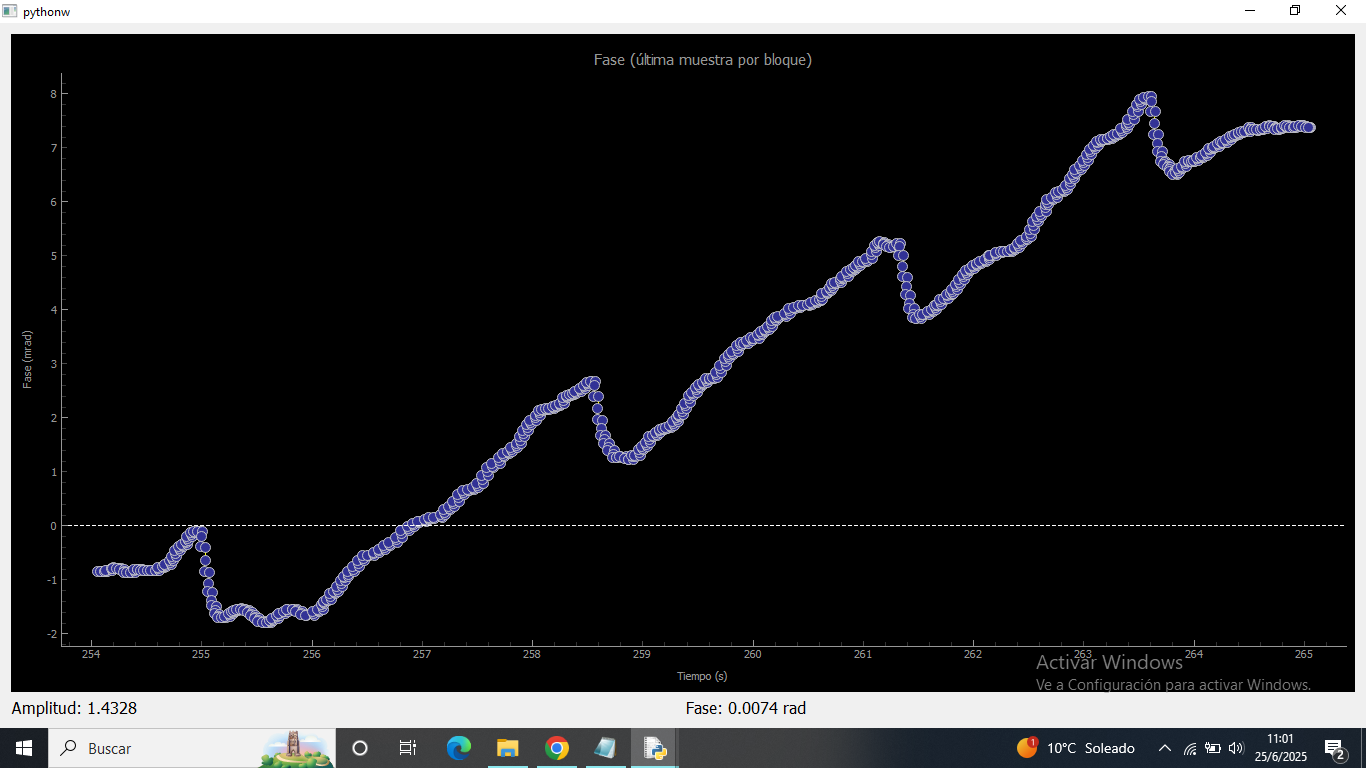
\includegraphics[width=0.98\textwidth]{Figures/23_06_2025/Saltos_cada_60_Hz_tiempo_real.png}
					\captionsetup{width=0.8\textwidth}
					\subcaption{Saltos.}
				\end{subfigure}
		\end{minipage}\begin{minipage}[c]{0.49\textwidth}
			\begin{subfigure}{\textwidth}
					\centering
					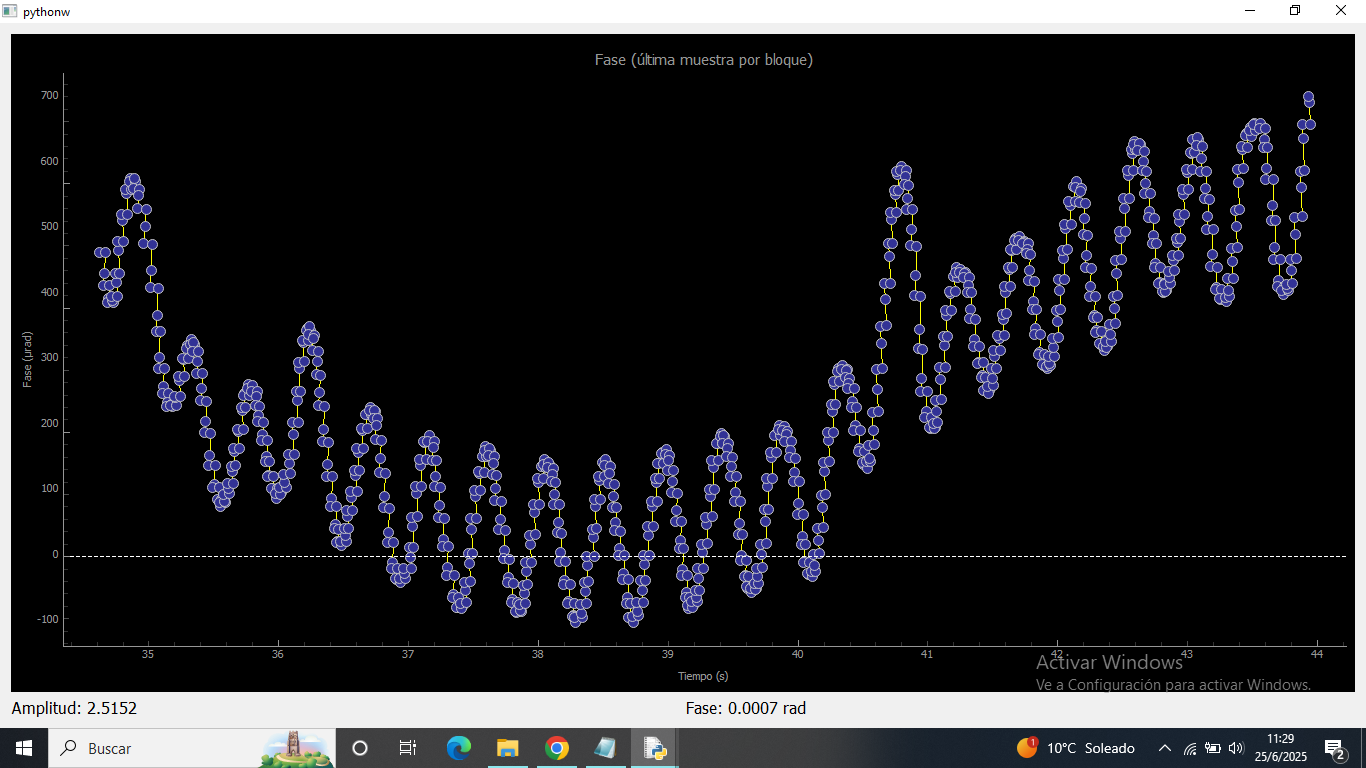
\includegraphics[width=0.98\textwidth]{Figures/23_06_2025/Oscilaciones_tiempo_Real.png}
					\captionsetup{width=0.8\textwidth}
					\subcaption{Oscilaciones.}
				\end{subfigure}
		\end{minipage}
	\caption{Artefactos del graficador en tiempo real, por no tener suficiente resolución la FFT para estimar correctamente la frecuencia de oscilación de la señal del generador (referencia).}
	\label{fig:artifacts_real_time_grapher_lock_in}
\end{figure}

Probamos barrer la frecuencia con la función de sweep del generador por si fuese la perilla, pero seguía pasando. 

Pensamos que era algo eléctrico por ser justo 60 Hz pero resultó ser el estimador de la frecuencia de la señal a partir de la FFT que tiene casualmente resolución de 500 kHz / 8192 puntos $\approx61$ Hz. Y después al bajar a 400 kHz con resolución 400 kHz / 8192 puntos $\approx$ 48 Hz el salto parecía ser cada 50 Hz. Además al guardar los datos y analizarlos a posteriori estos artefactos no ocurrían.

\subsection*{Agua del Canal de Ingeniería.}
Para esto hice un par de cosas. Por un lado la calibración con el tornillo micrométrico que se ve a continuación:


\begin{figure}[th!]
	\centering
	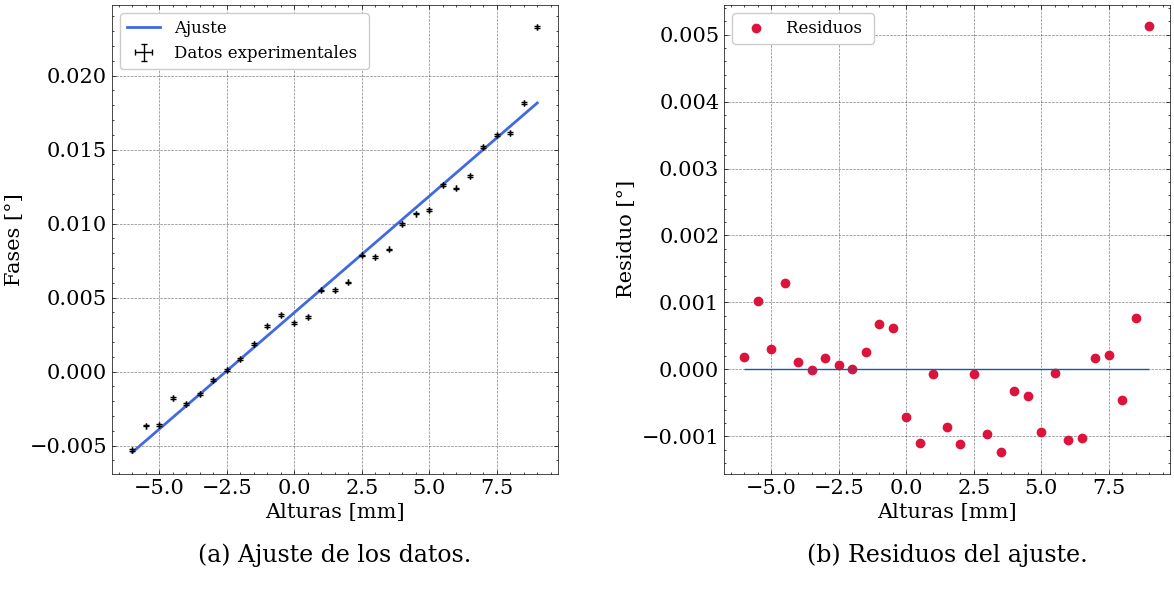
\includegraphics[width=0.87\linewidth]{Figures/23_06_2025/Ajuste_canal}
	\caption{Calibración de fase contra altura para el agua del canal en un vaso de vidrio.}
	\label{fig:ajustecanal}
\end{figure}

Los parámetros del ajuste fueron: $R^2=0.97448$,	$\chi_\nu^2=383.93621$,	$m = (0.00157 \pm 0.00005)\; mm/°$,	$b = (0.0040 \pm 0.0002)\; mm$.

Y algunas mediciones forzado el líquido del vaso, ya sea de adelante para atrás o rotando, y como se ve a continuación, el sensor funciona razonablemente bien.


\begin{figure}[th!]
	\centering
	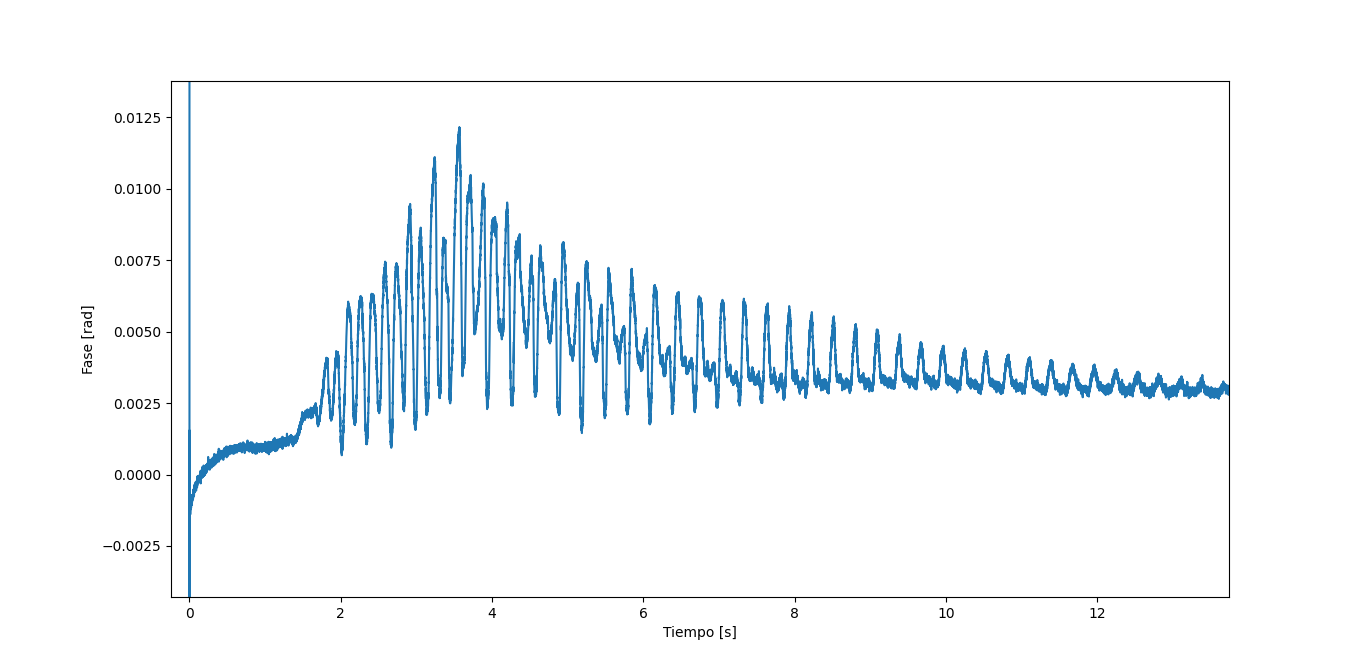
\includegraphics[width=0.78\linewidth]{Figures/23_06_2025/Forzado_VASO_CANAL}
	\caption{Forzado de adelante para atrás del vaso. }
	\label{fig:forzadovasocanal}
\end{figure}

\begin{figure}[th!]
	\centering
	\includegraphics[width=0.78\linewidth]{Figures/23_06_2025/Rotación_VASO_CANAL.png}
	\caption{Rotación del vaso. Hacia el final se nota un salto de fase cuando dejo de tocar el vaso.}
	\label{fig:rotadovasocanal}
\end{figure}


Para terminar también medí el ruido tocando y sin tocar.


\subsection*{Forzado en la cuba grande.}
Por último armamos con Manu para medir en la cuba grande como se ve en la foto:

\begin{figure}[th!]
	\centering
	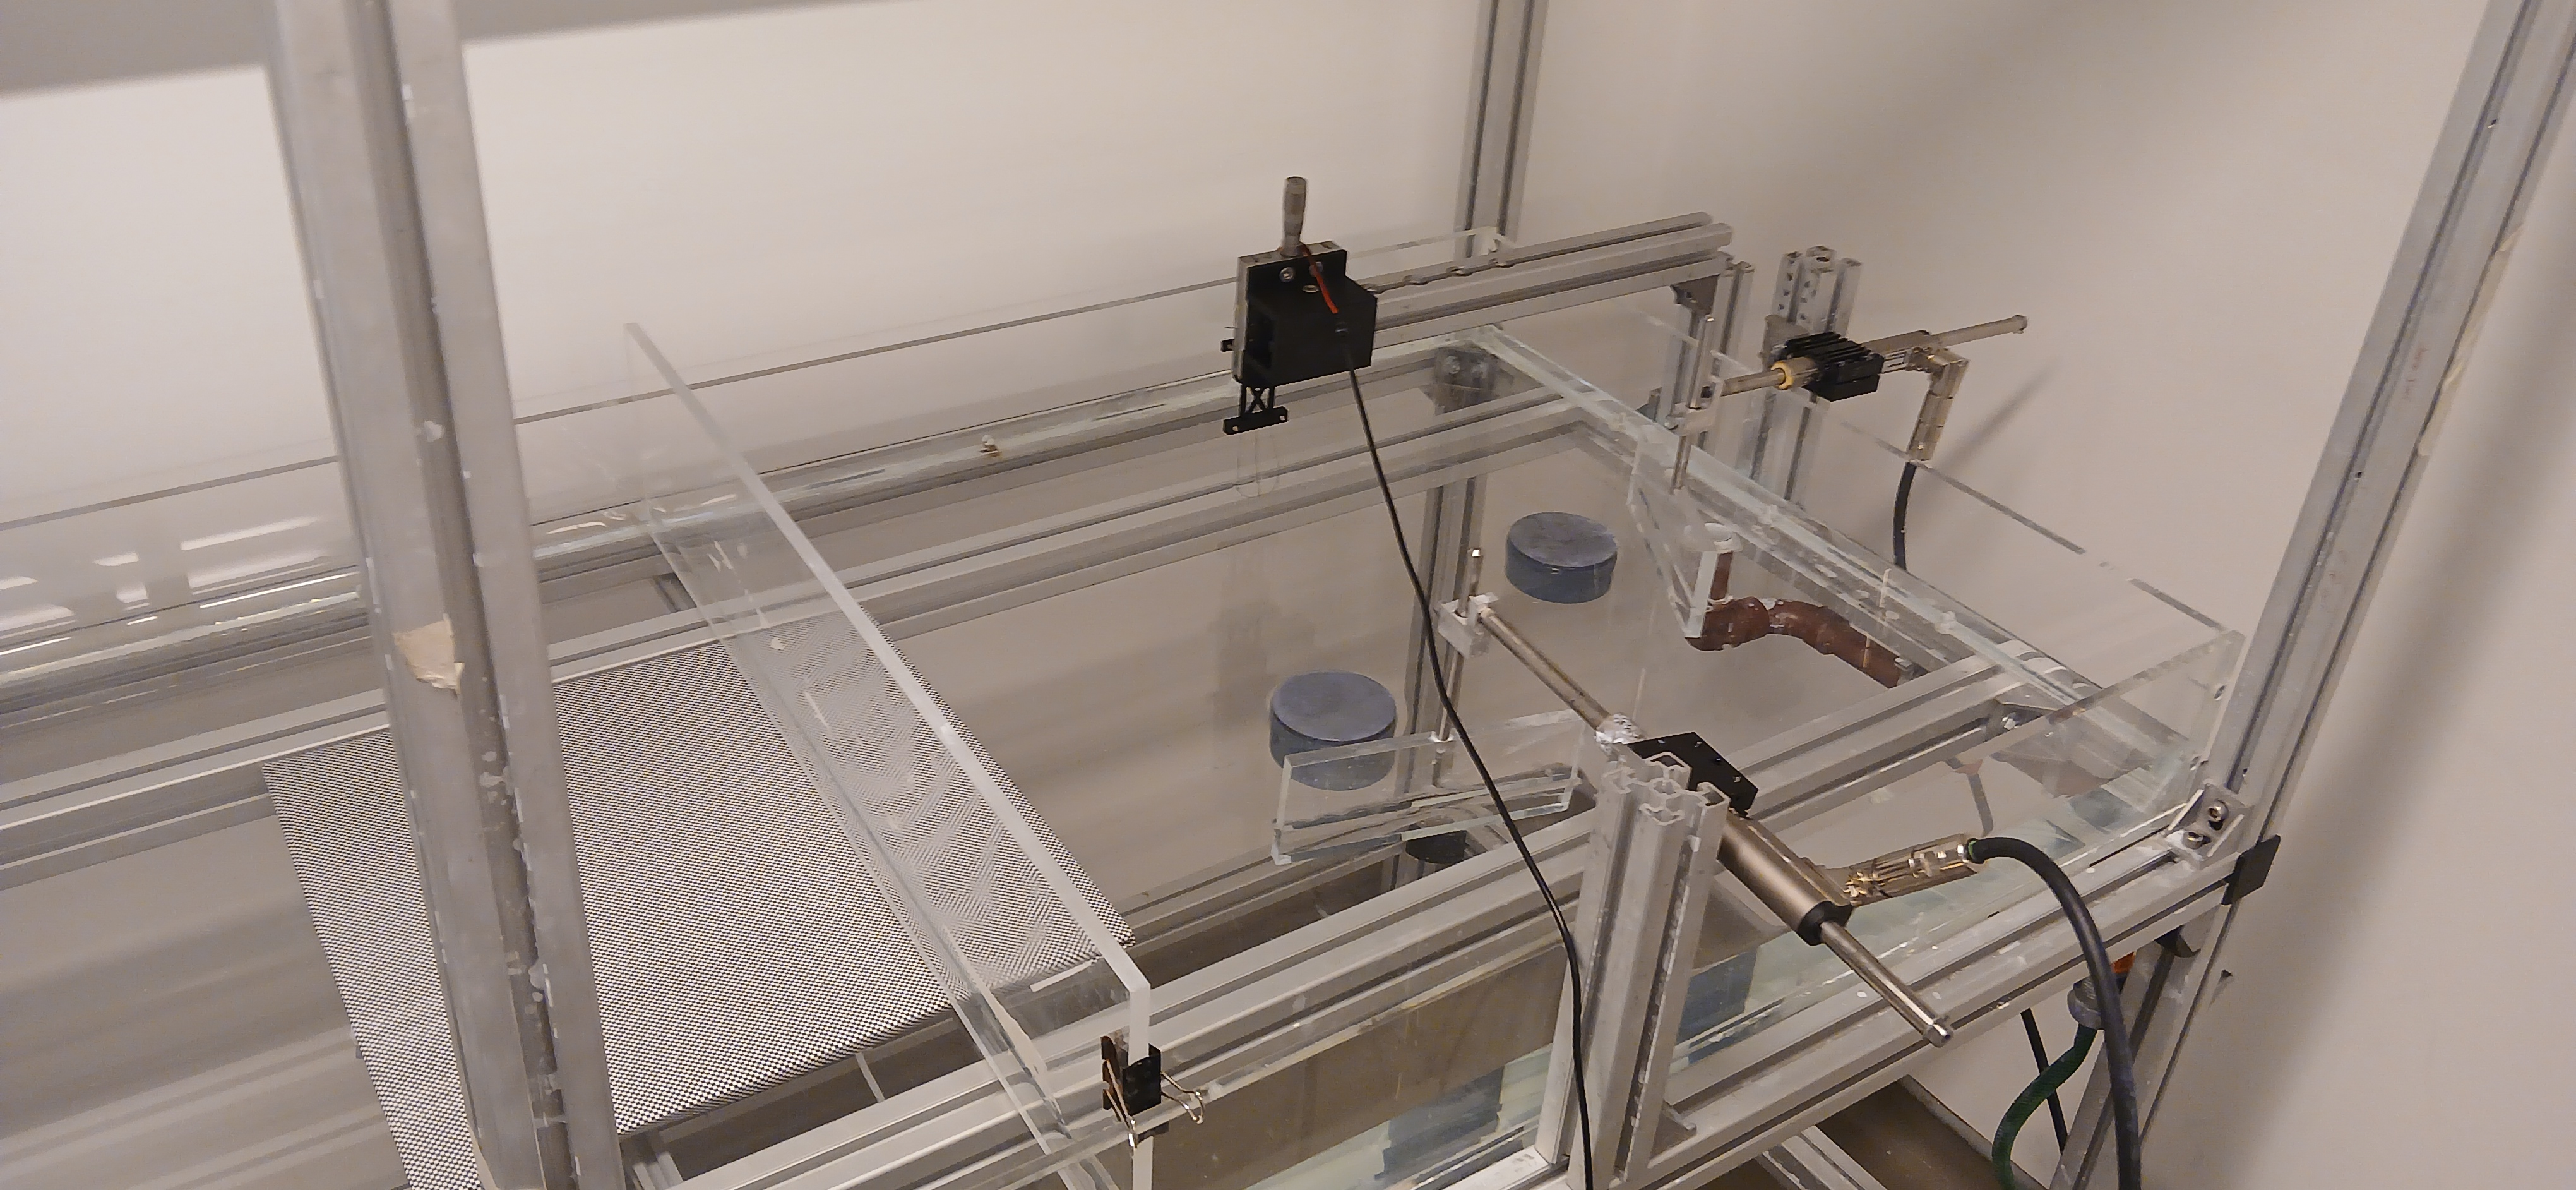
\includegraphics[width=0.780257\linewidth]{Figures/23_06_2025/Cuba_forzado_y_sensor}
	\caption{Setup para medir en la cuba grande wave turbulence con el sensor capacitivo. } % $$ ia
	\label{fig:cubaforzadoysensor}
\end{figure}


Usamos uno y dos motores, con dos de los obstáculos para romper los modos normales de la cuba y la barrera para evitar perder energía lejos del sensor, que pusimos con un perfil de aluminio lo más lejos de las paredes posible.

\begin{figure}[!ht]
	\centering
	\includegraphics[width=0.7065810257\linewidth]{"Figures/23_06_2025/Forzado de los motores"}
	\caption{Curva del forzado de los motores (tiempo total 30 s, 8192 puntos).}
	\label{fig:forzado-de-los-motores}
\end{figure}


Para los motores usamos uno de los forzados que ya estaban precargados, ya que no teníamos mucho tiempo. 

Aunque en el futuro probablemente querramos usar amplitud constante entre 0 y 4 Hz (o ir variando hasta 5 o 6 Hz) en vez de ruido como ahora.

\begin{figure}[th!]
	\centering
	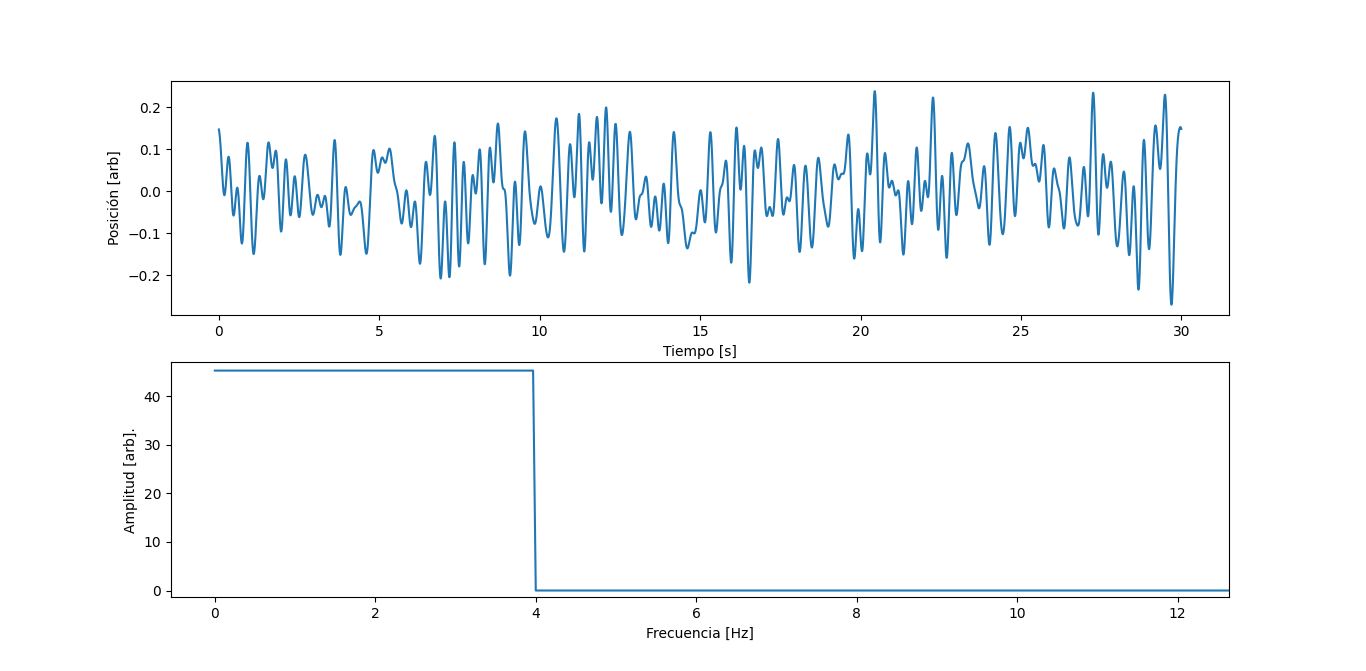
\includegraphics[width=0.7065810257\linewidth]{Figures/23_06_2025/Amplitud_constante}
	\caption{Próximos forzados a probar en el motor (Tiempo total 30 s, 8192 puntos). Es importante que sea periódica para evitar saltos en los motores.} % aa 
	\label{fig:amplitudconstante}
\end{figure}

Tomamos las siguientes mediciones para uno y dos motores prendidos: 
\begin{itemize}
	\item Estacionario. 
	\item Decaimiento al apagar el motor. 
	\item Ruido con el/los motores apagados.
\end{itemize}


\section{Viernes 27/06/2025}  
Me centré en continuar con el análisis de los datos de la cuba grande del Miércoles pasado. Reescribí el código para nuevamente pasar los valores anteriores del filtro exponencial a la ventana siguiente, para así solo procesar de a pedazos el archivo completo, leyendo cada uno con memmap de numpy, y así no sobrecargar la memoria. Además como son millones y millones de puntos literalmente optimicé el filtro exponencial con numba para que no tarde tanto, al ser simplemente un loop.            

\begin{figure}[th!]
	\centering
	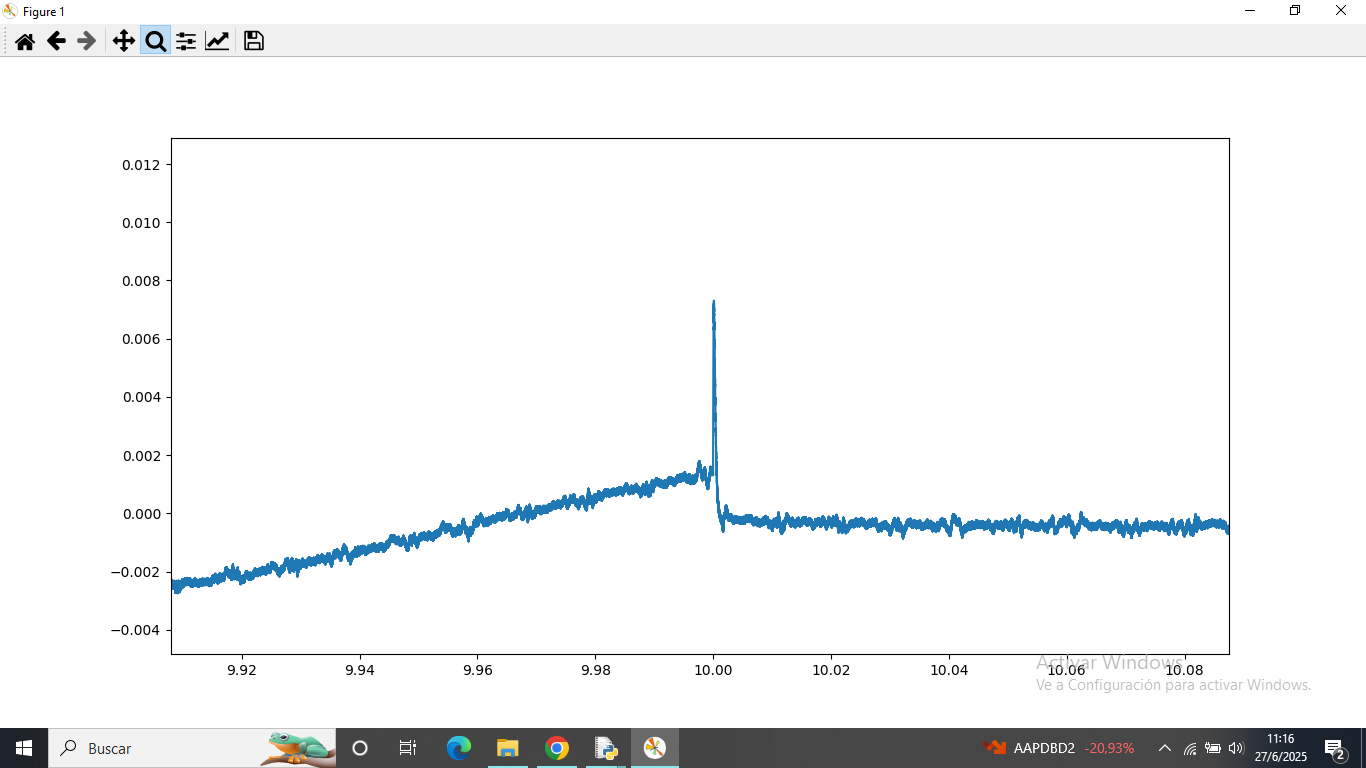
\includegraphics[width=0.429567\linewidth]{Figures/23_06_2025/Salto_temporal_entre_ventanas}
	\caption{Salto entre ventanas al analizar una medición larga con lock-in por partes.}
	\label{fig:saltotemporalentreventanas}
\end{figure}


Sin embargo aún al pasar los valoes anteriores se da un salto en la fase, que imagino tiene que ver con los últimos puntos de la referencia que hacen cosas raras con el resampleo y shift de 90°, ya que analizando ese pedazo en continuo los saltos no aparecen, así que no es algo de la señal. 


Además de las alturas procesadas hago la FFT y corto todos los puntos con frecuencia mayor a la de corte del lock-in ya que dan 0 y son información redundante, y es mejor esto que simplemente tomar uno de cada x puntos subsampleando. Para esto, hay que recalcular la tira de tiempos.

\begin{figure}[th!]
	\centering
	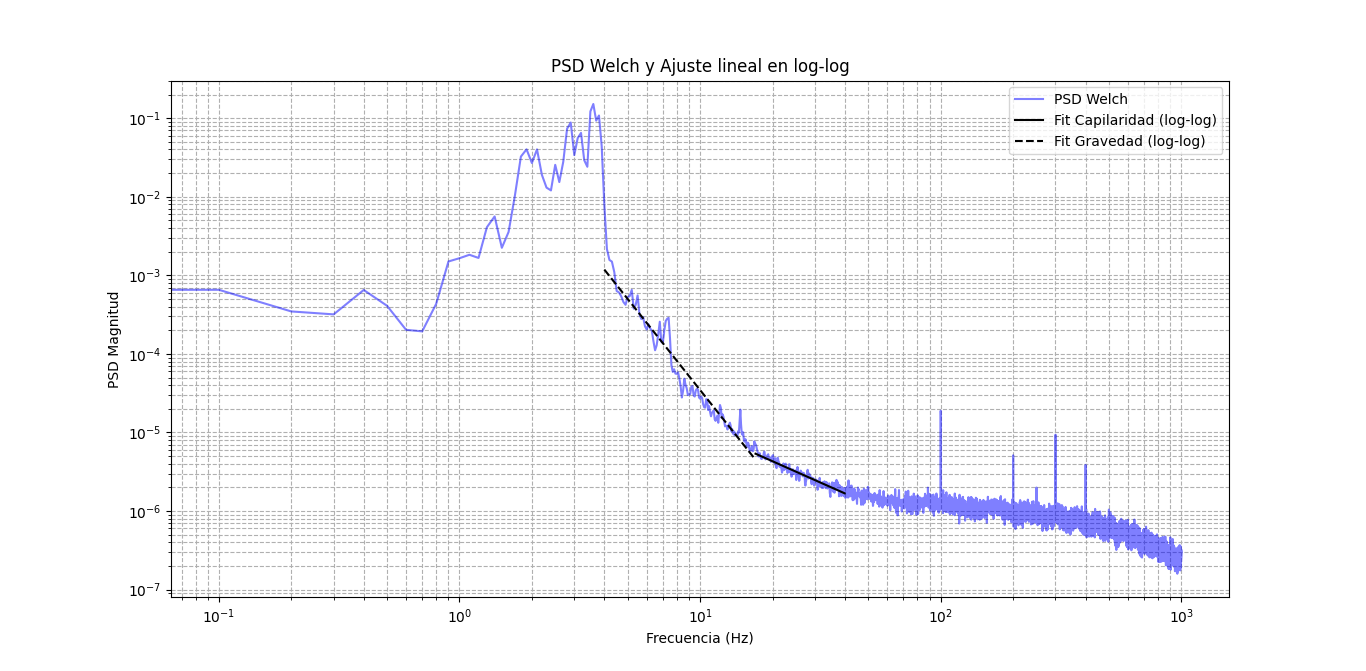
\includegraphics[width=0.87\linewidth]{Figures/23_06_2025/Espectro_dos_motores_cuba_grande}
	\caption{Espectro de la cuba grande con dos motores prendido, usando Welch para la tira completa. Ventana de 10 s y overlap de 9.1 s.}
	\label{fig:espectrodosmotorescubagrande}
\end{figure}

Las pendientes del ajustes son: 
\begin{itemize}
	\item Gravedad: $m=-3.852$ rad$^2$/Hz$^2$, $b-=1.398$ rad$^2$/Hz. 
	\item Capilar: $m=-0.748$ rad$^2$/Hz$^2$, $b=-10.349$ rad$^2$/Hz.
\end{itemize}

\begin{figure}[th!]
	\centering
	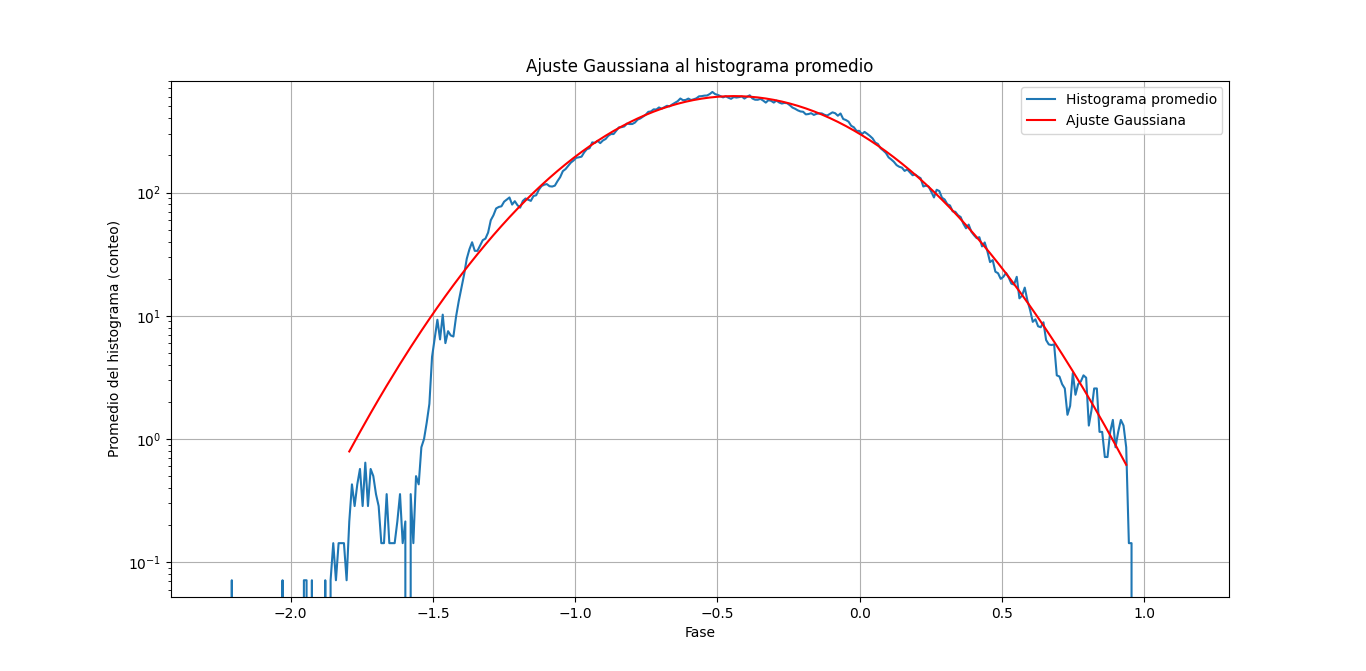
\includegraphics[width=0.87\linewidth]{Figures/23_06_2025/PDFS_dos_motores_cuba_grande}
	\caption{PDFs para los dos motores prendidos y un ajuste gaussiano de los mismos.}
	\label{fig:pdfsdosmotorescubagrande}
\end{figure}

Quedaría calcular la correlación entre varios pedazos de 30 segundos de la señal ya que se repite el movimiento del motor periódicamente en este caso, y bueno, analizar el resto de cosas. % ´´odi a
